\chapter{Aplicação Desenvolvida}

\section{UML de Componentes}

\begin{figure}[h]
  \caption{Componentes do processo SW}\label{fig:componentssw}
  \centering
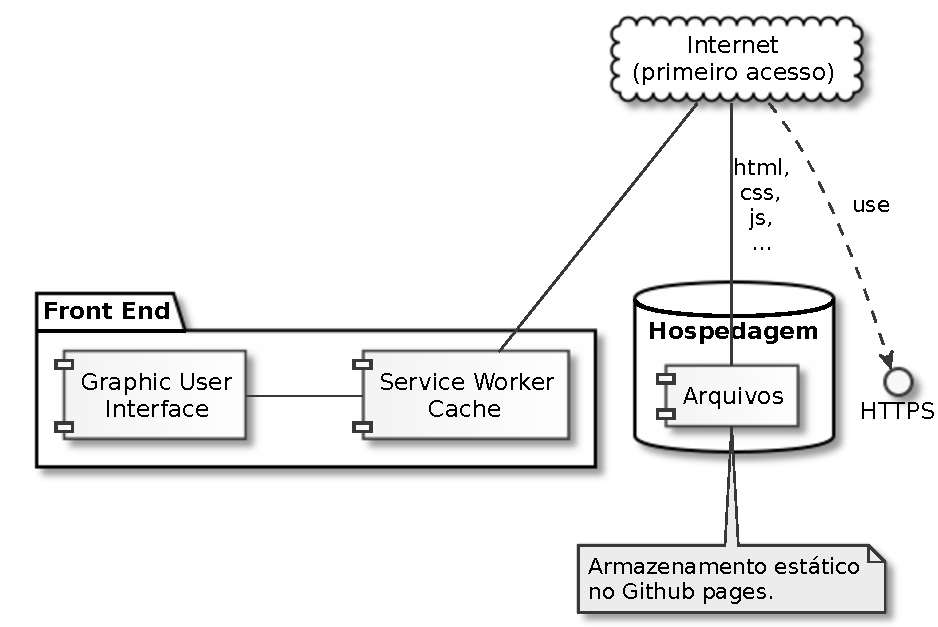
\includegraphics[keepaspectratio]{figures/components-sw.pdf}
  \caption*{\footnotesize Fonte: Produção do autor, 2016.}
\end{figure}

\begin{figure}[h]
  \caption{Componentes da tradução}\label{fig:componentsrun}
  \centering
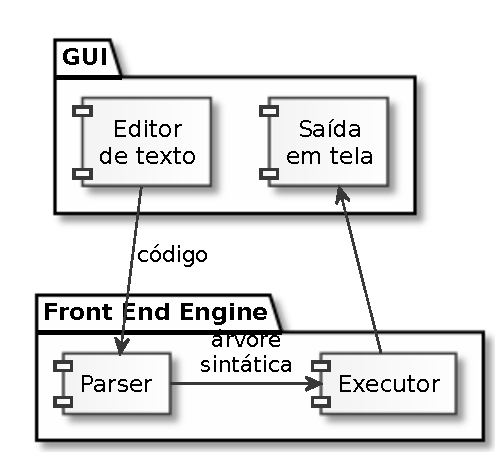
\includegraphics[keepaspectratio]{figures/components-run.pdf}
  \caption*{\footnotesize Fonte: Produção do autor, 2016.}
\end{figure}

\begin{quadro}[h]
\centering
  \caption{Árvore sintática gerada}\label{qua:sintaxtree}
\begin{lstlisting}[style=json,frame=single]
{
  "type": "Program",
  "start": 0,
  "end": 61,
  "body": [
    {
      "type": "PrintStatement",
      "start": 19,
      "end": 53,
      "print": {
        "type": "CallPrint",
        "start": 27,
        "end": 52,
        "arguments": {
          "type": "Literal",
          "start": 27,
          "end": 52,
          "value": "Aprendendo Algoritmo!!!",
          "raw": "\"Aprendendo Algoritmo!!!\""
        }
      }
    }
  ],
  "id": {
    "type": "Identifier",
    "start": 5,
    "end": 16,
    "name": "algoritmo11"
  }
}
\end{lstlisting}
  \caption*{\footnotesize Fonte: Produção do autor.}
\end{quadro}

\begin{figure}[h]
  \caption{Interface Desktop}\label{fig:interfacedesktop}
  \centering
  \setlength{\fboxsep}{0pt}%
\setlength{\fboxrule}{1pt}%
\fbox{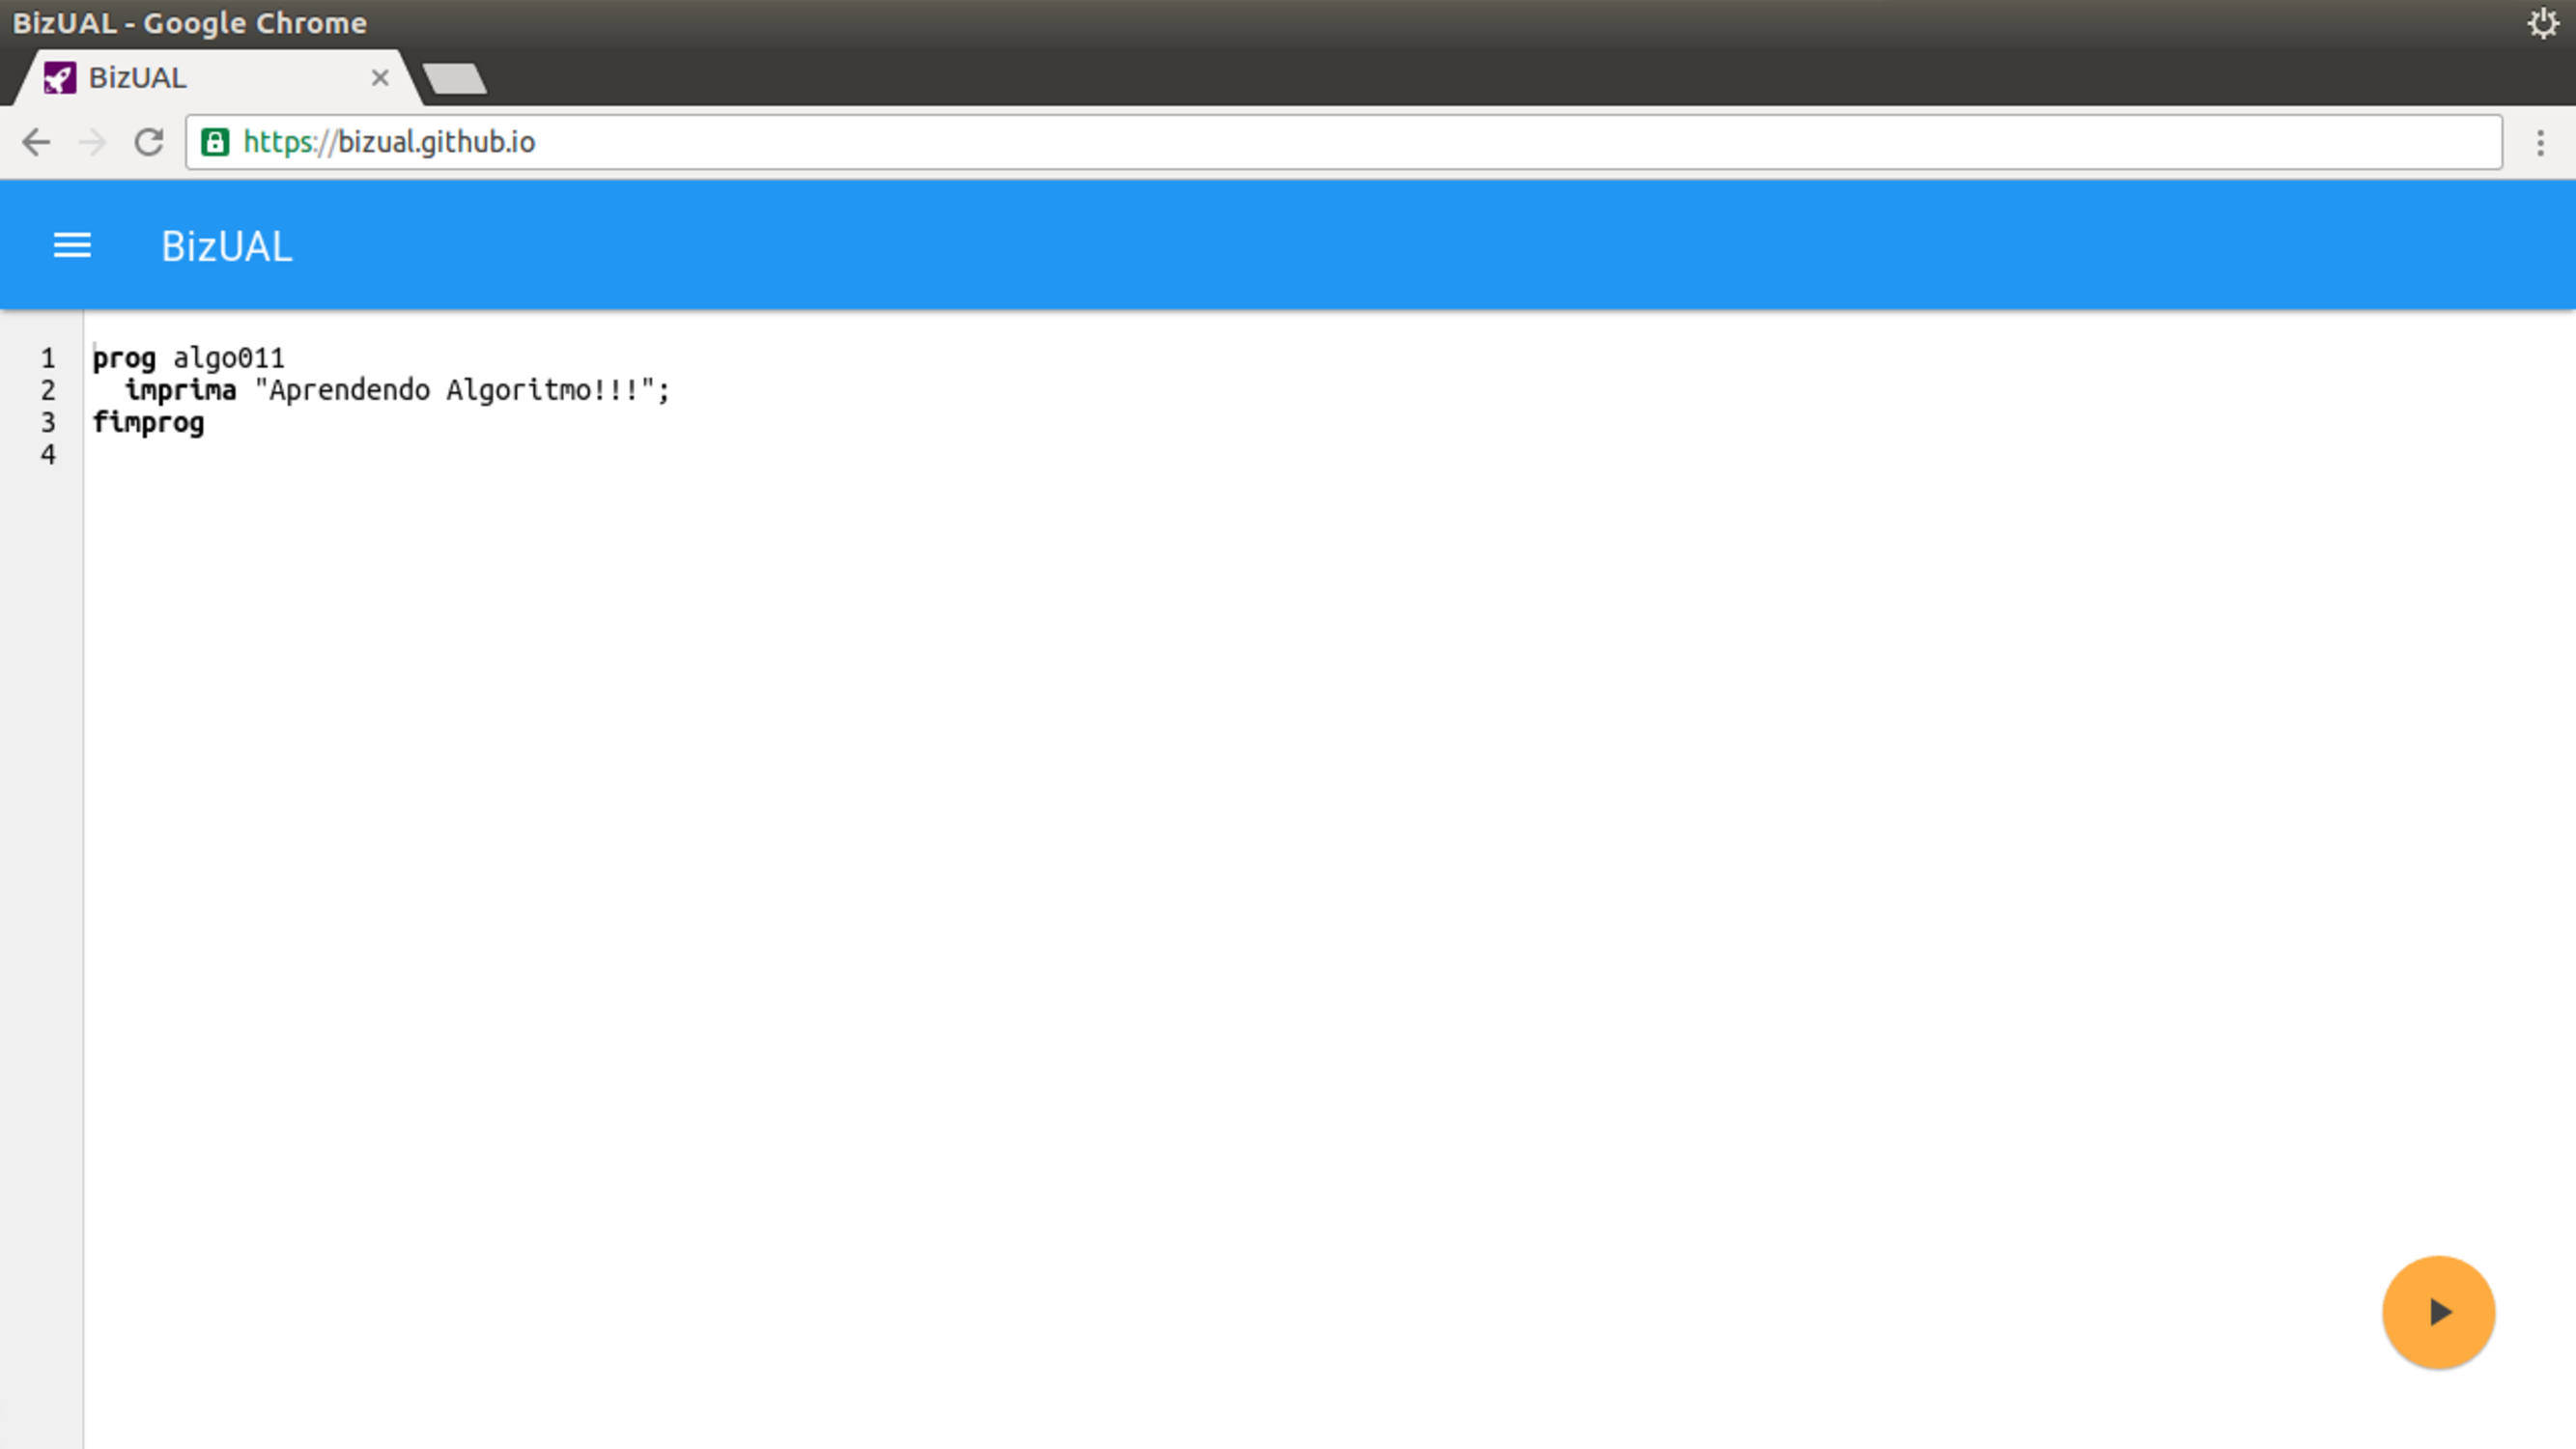
\includegraphics[width=\textwidth,keepaspectratio]{figures/bizual-desktop.pdf}}
  \caption*{\footnotesize Fonte: Produção do autor, 2016.}
\end{figure}

\begin{figure}[h]
  \caption{Interface Smartphone}\label{fig:interfacesmartphone}
  \centering
  \setlength{\fboxsep}{0pt}%
\setlength{\fboxrule}{1pt}%
\fbox{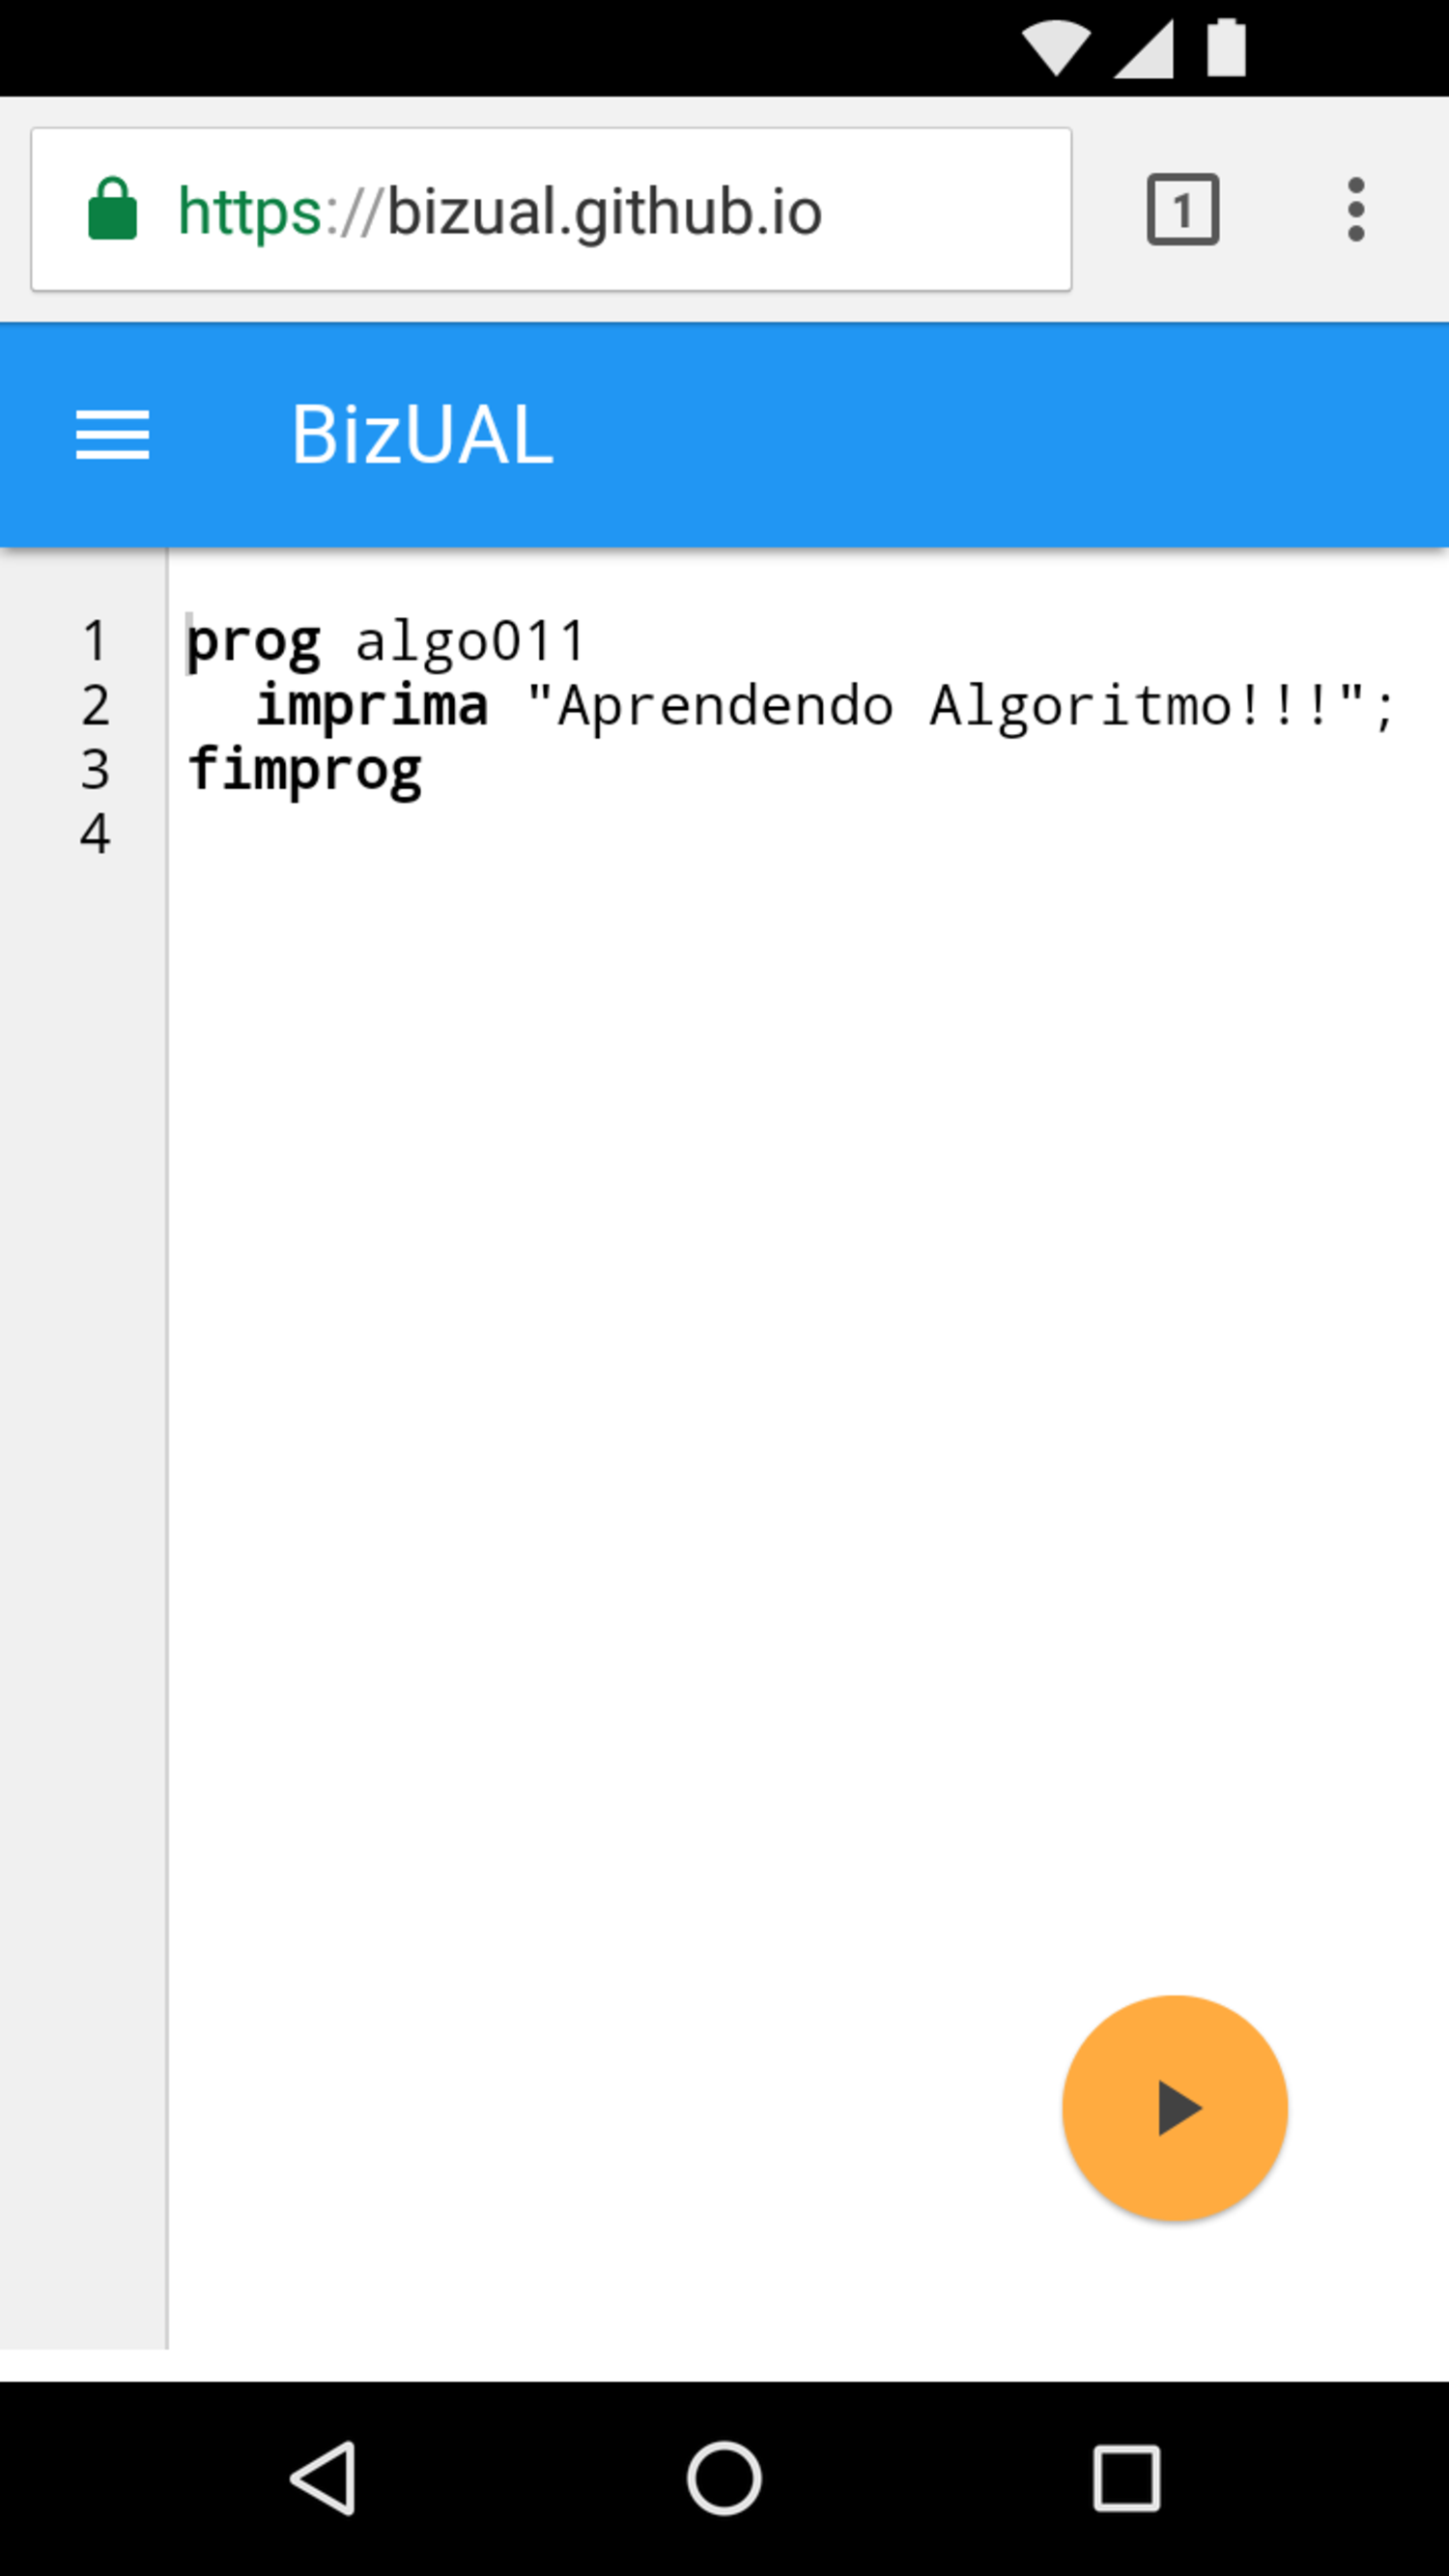
\includegraphics[width=.5\textwidth,keepaspectratio]{figures/bizual-smartphone.pdf}}
  \caption*{\footnotesize Fonte: Produção do autor, 2016.}
\end{figure}

\begin{figure}[h]
  \caption{Interface Smartphone Paisagem}\label{fig:interfacesmartphoneh}
  \centering
  \setlength{\fboxsep}{0pt}%
\setlength{\fboxrule}{1pt}%
\fbox{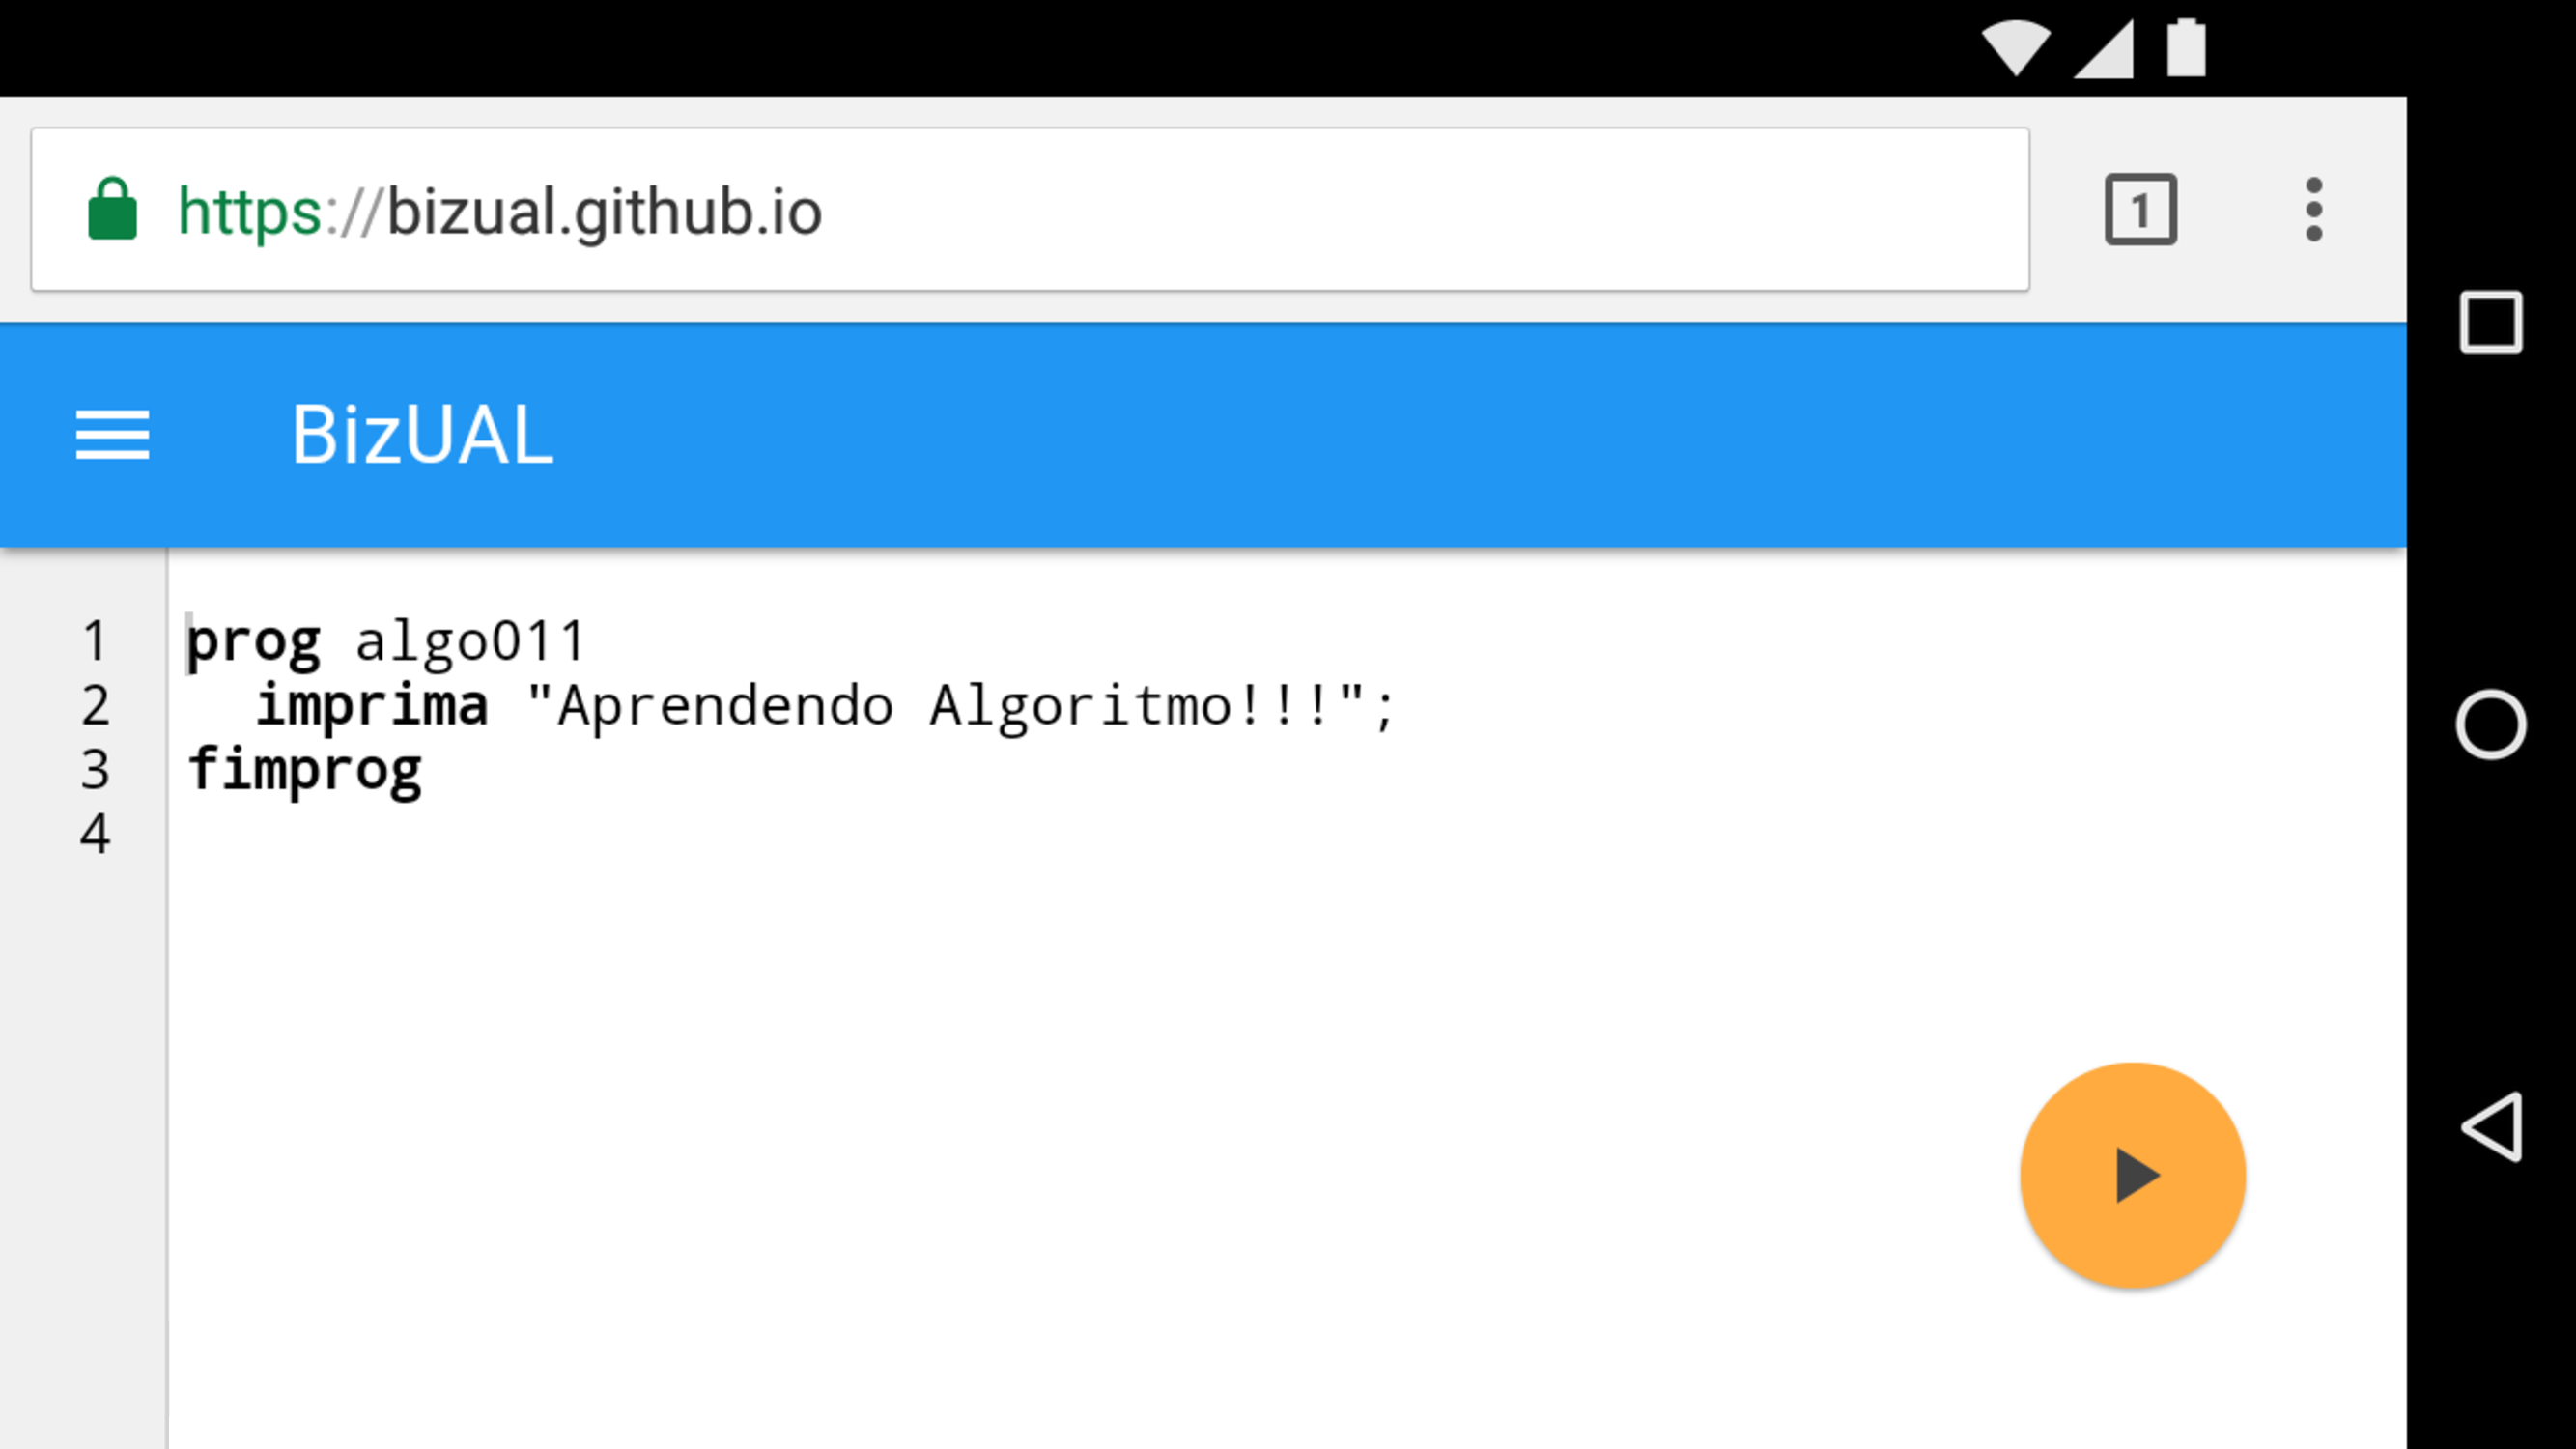
\includegraphics[width=\textwidth,keepaspectratio]{figures/interface-mobile-h.pdf}}
  \caption*{\footnotesize Fonte: Produção do autor, 2016.}
\end{figure}

\begin{figure}[h]
  \caption{Execução Desktop}\label{fig:executiondesktop}
  \centering
  \setlength{\fboxsep}{0pt}%
\setlength{\fboxrule}{1pt}%
\fbox{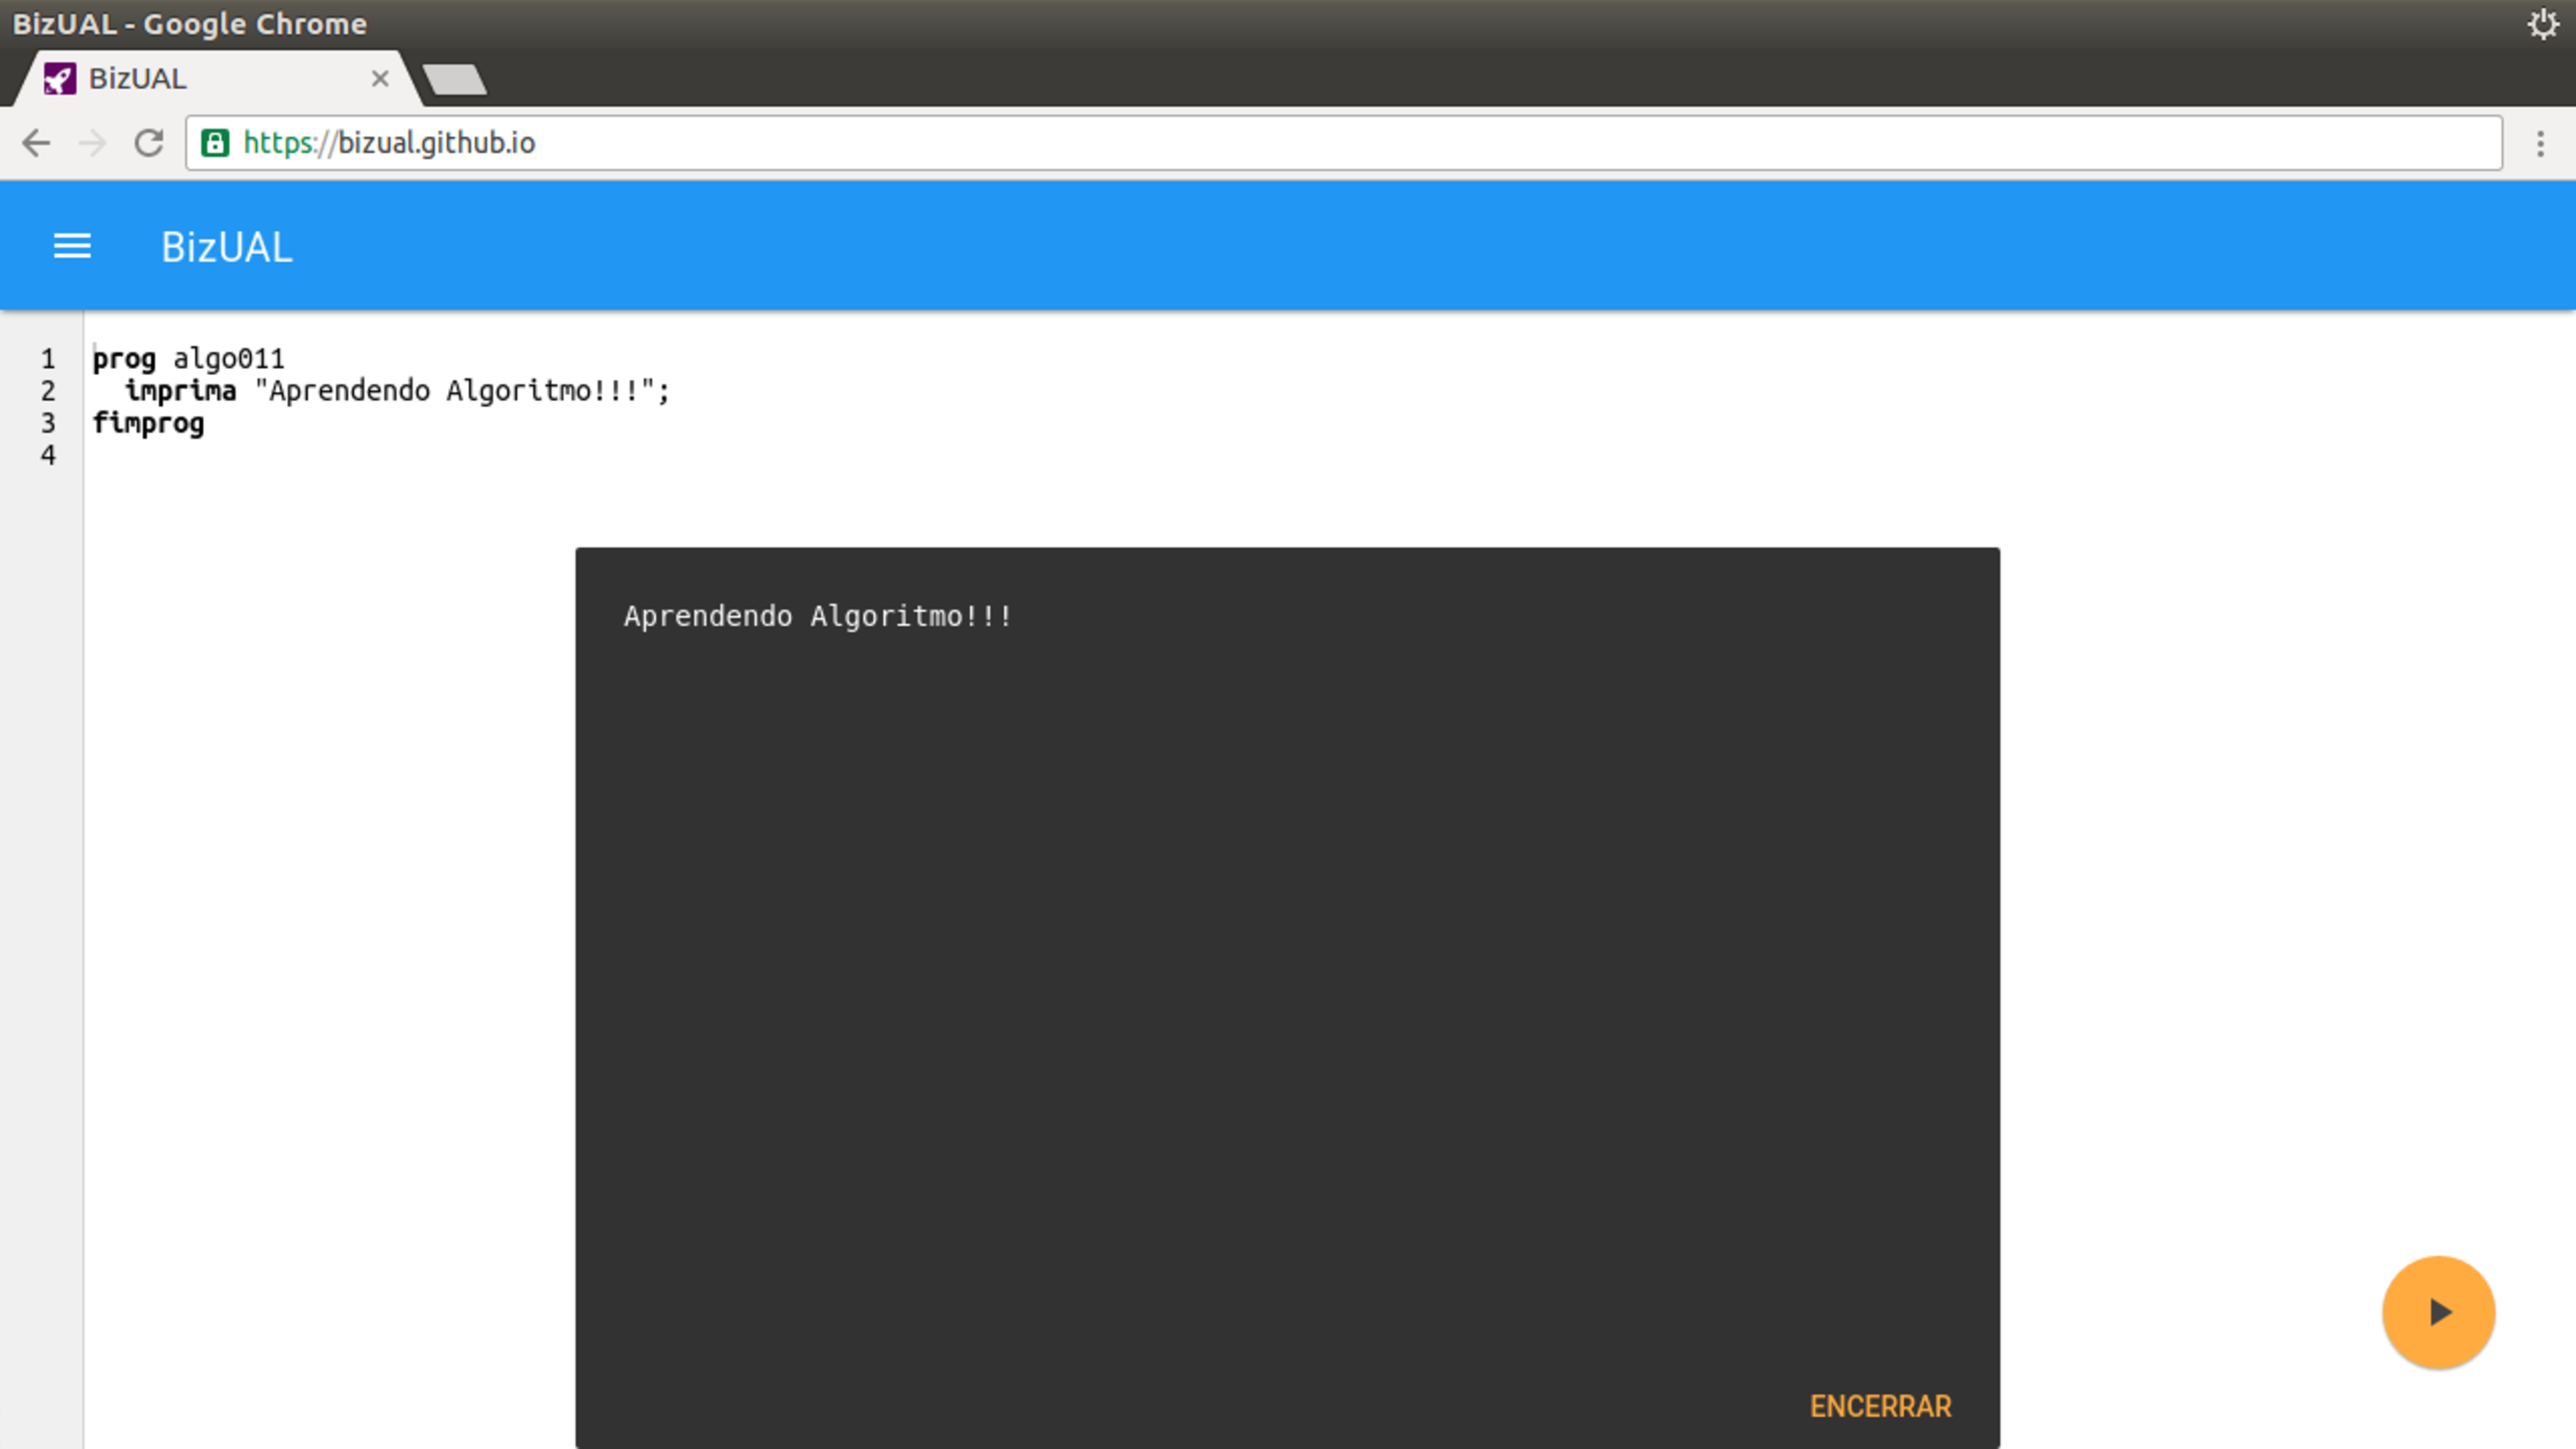
\includegraphics[width=\textwidth,keepaspectratio]{figures/execucao-desktop.pdf}}
  \caption*{\footnotesize Fonte: Produção do autor, 2016.}
\end{figure}

\begin{figure}[h]
  \caption{Execução Smartphone}\label{fig:executionsmartphone}
  \centering
  \setlength{\fboxsep}{0pt}%
\setlength{\fboxrule}{1pt}%
\fbox{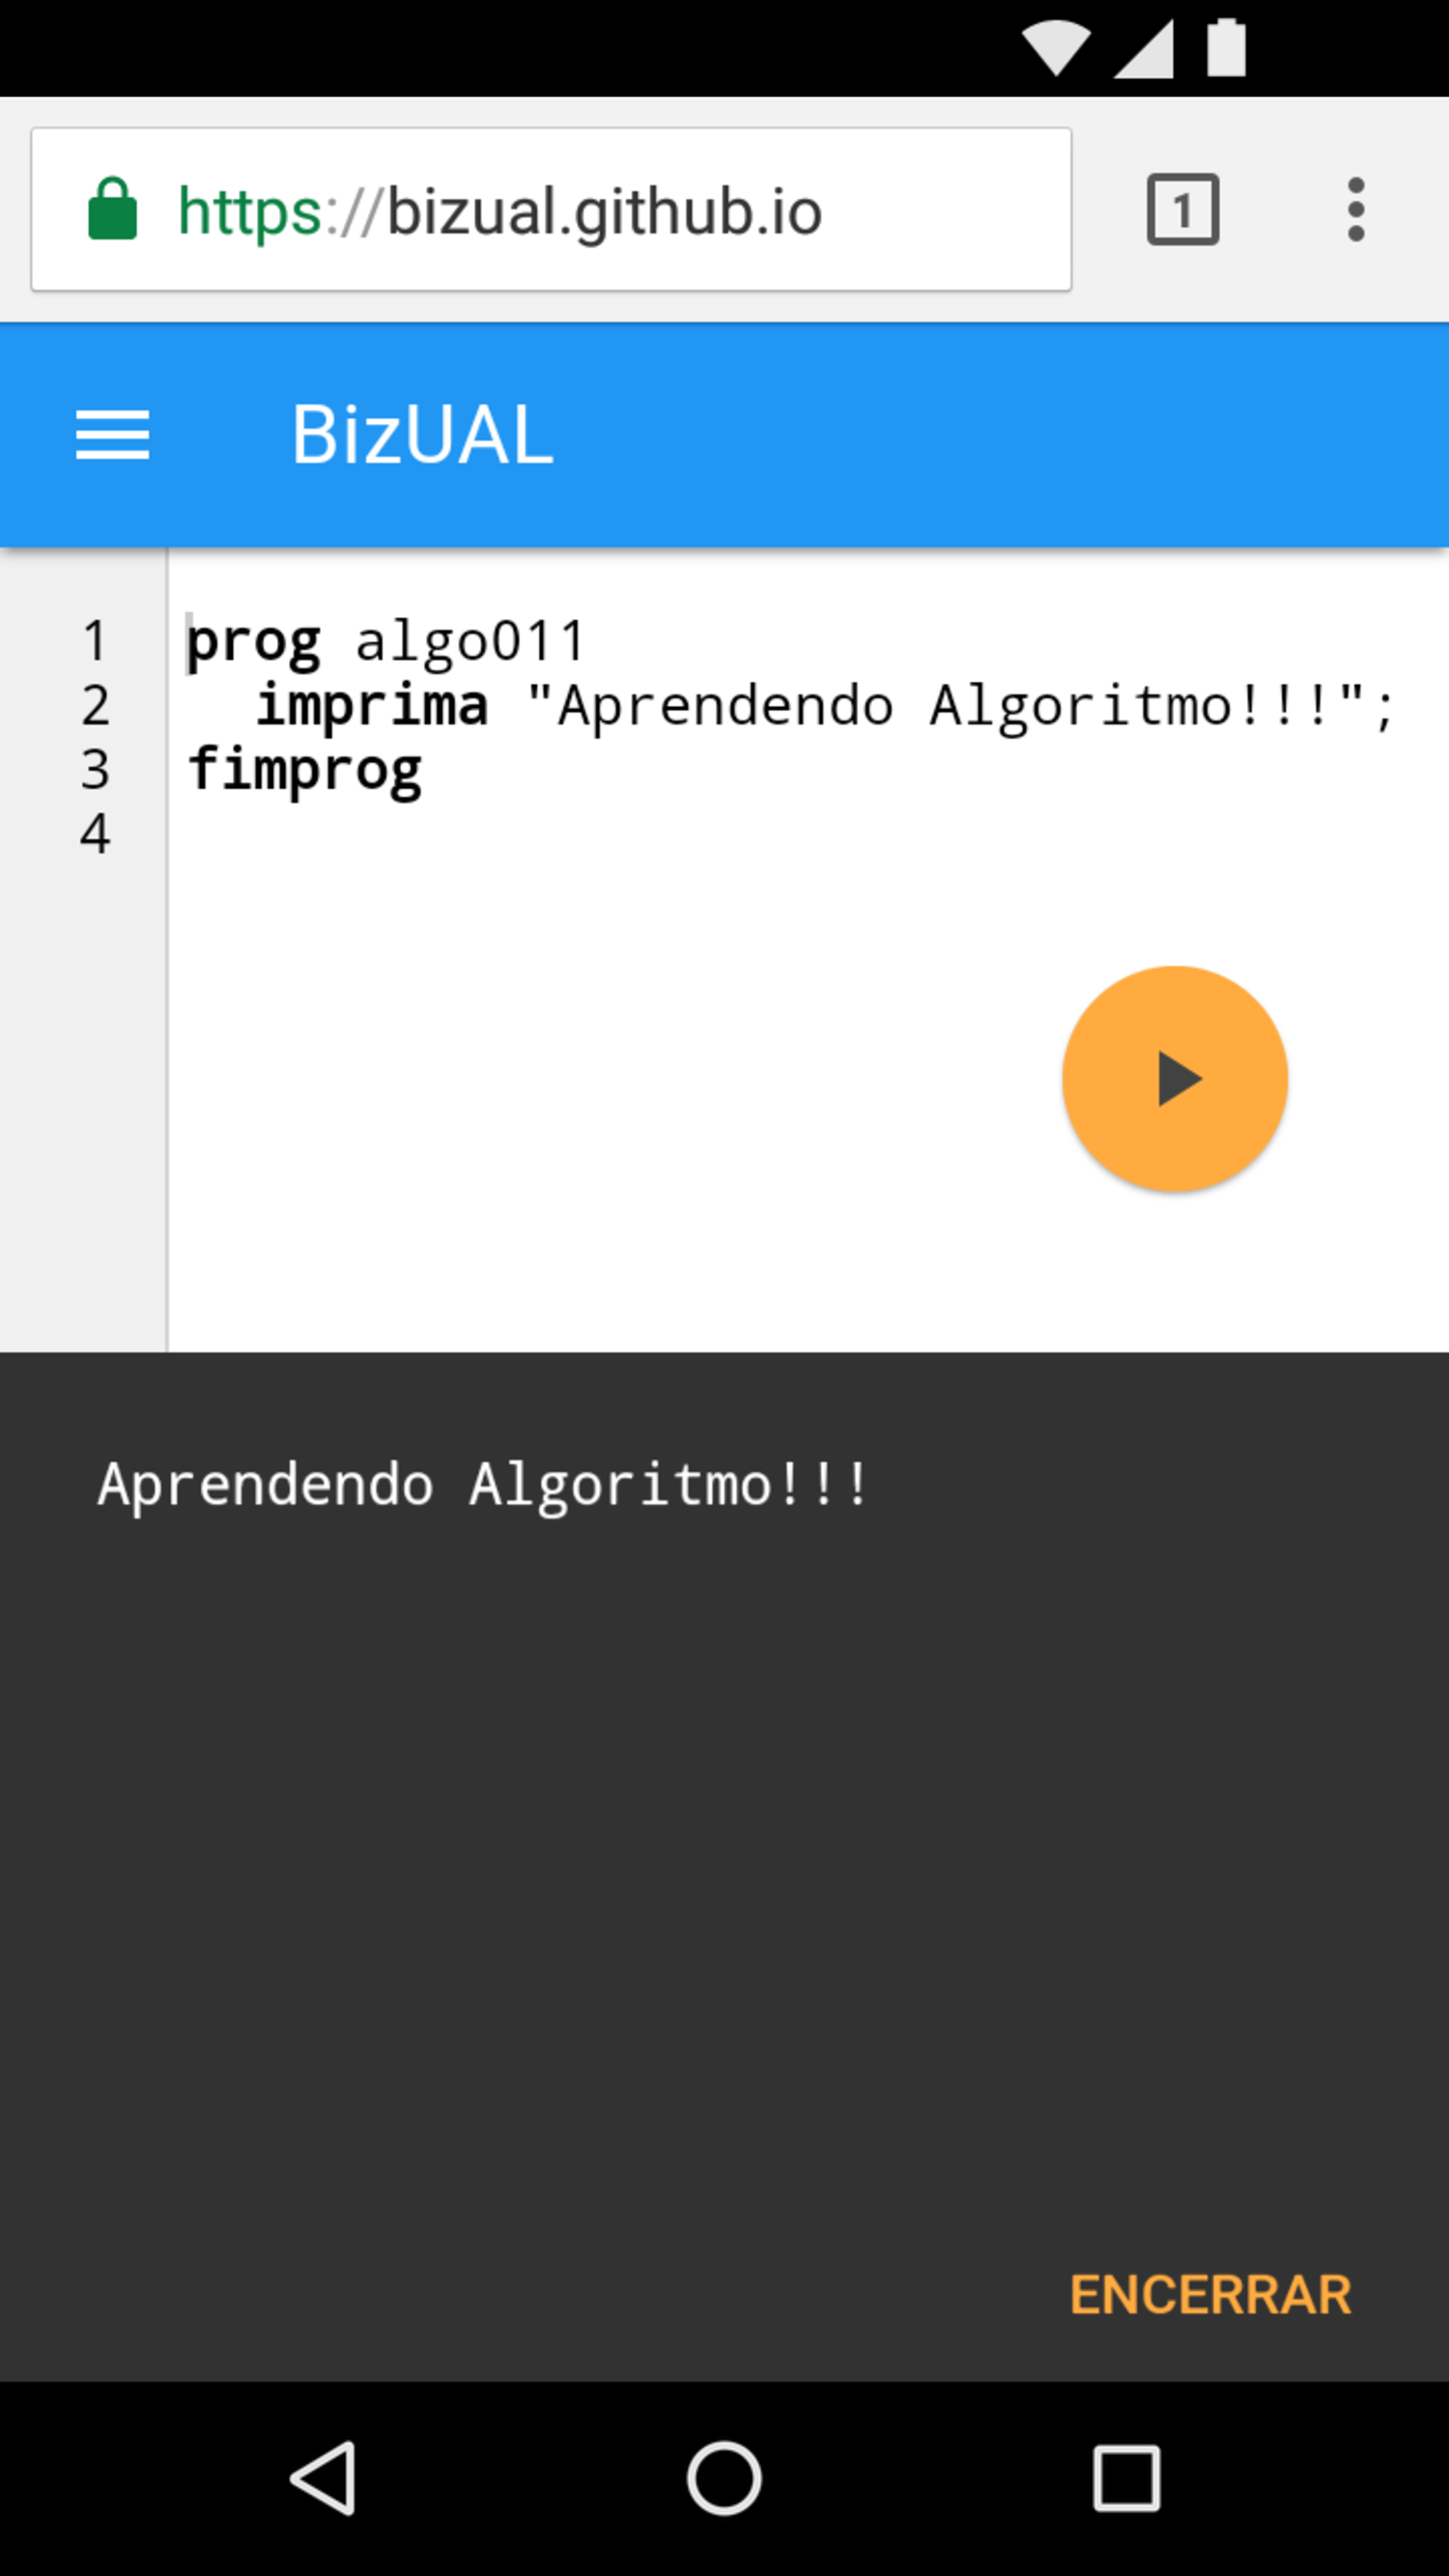
\includegraphics[width=.5\textwidth,keepaspectratio]{figures/execution-mobile-v.pdf}}
  \caption*{\footnotesize Fonte: Produção do autor, 2016.}
\end{figure}

\begin{figure}[h]
  \caption{Execução Smartphone}\label{fig:executionsmartphoneh}
  \centering
  \setlength{\fboxsep}{0pt}%
\setlength{\fboxrule}{1pt}%
\fbox{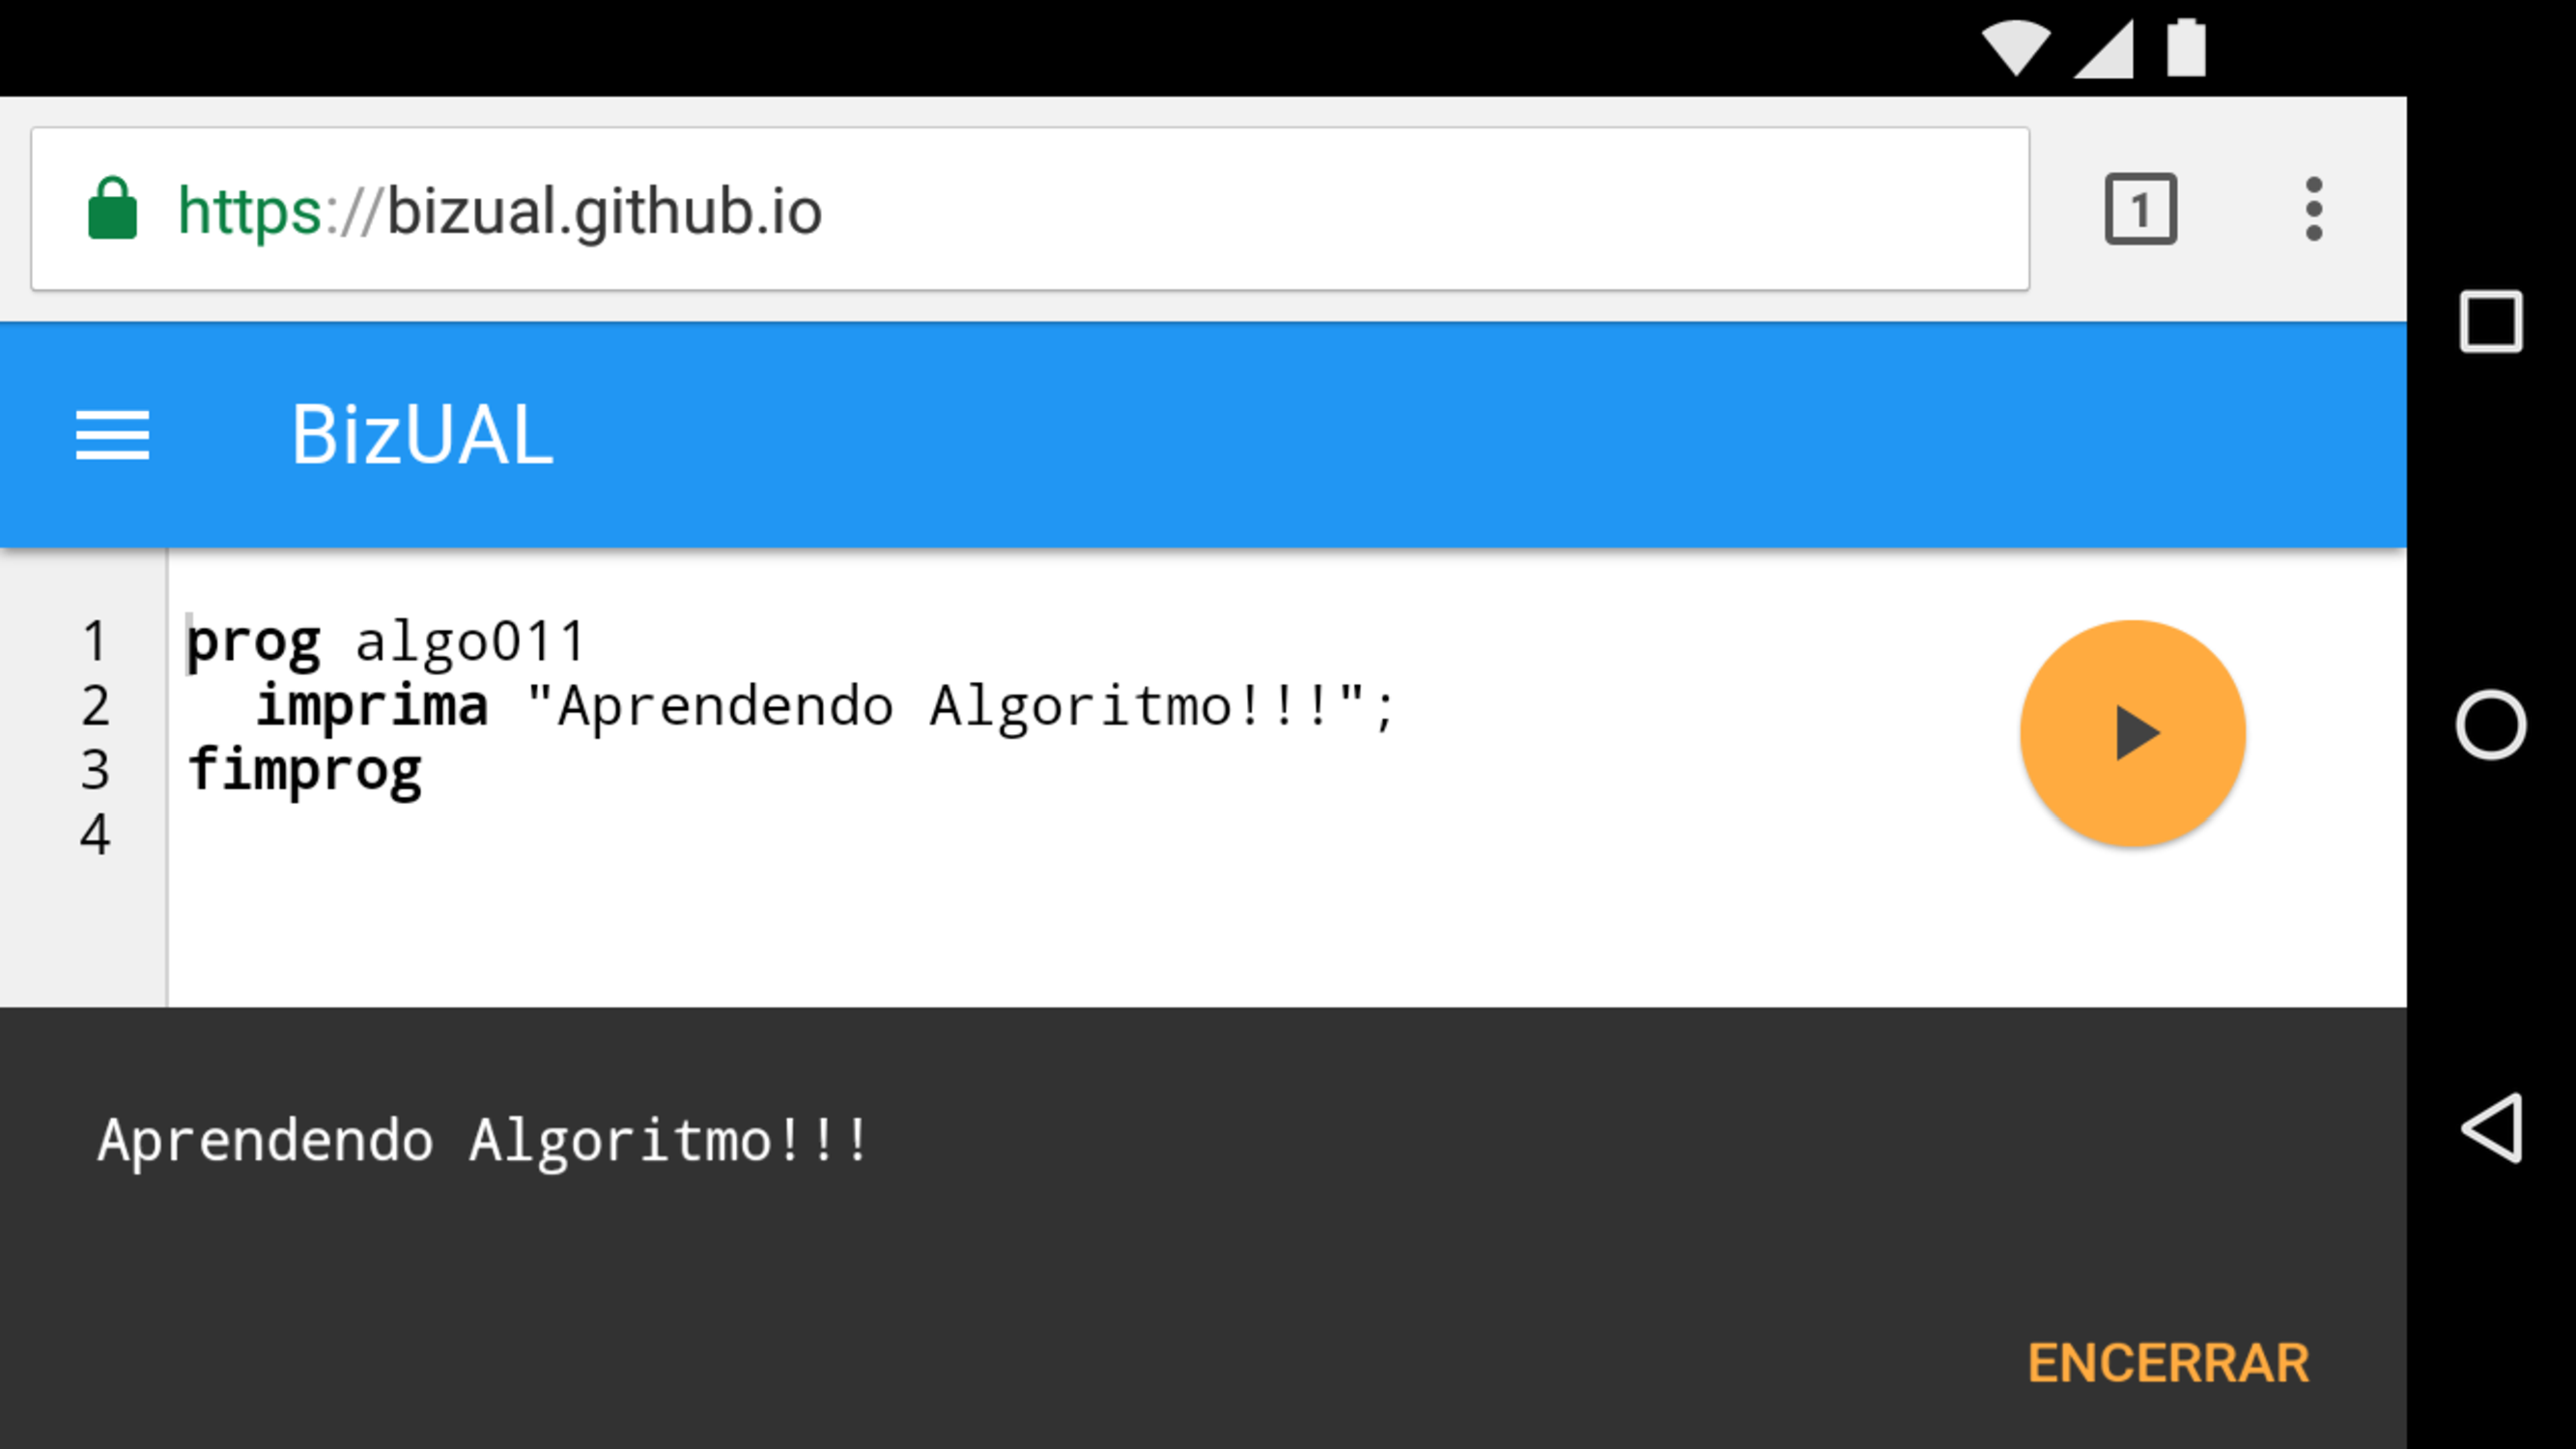
\includegraphics[width=\textwidth,keepaspectratio]{figures/execution-mobile-h.pdf}}
  \caption*{\footnotesize Fonte: Produção do autor, 2016.}
\end{figure}

